\vspace{0.5cm}
\begin{figure}[htb!]
\centering
 \subfloat[]{%
 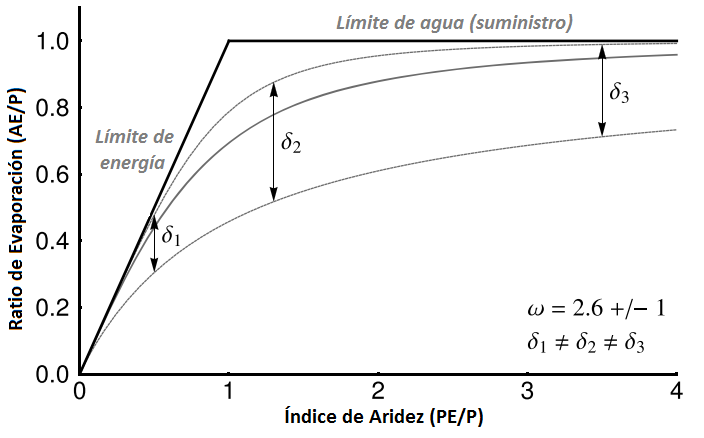
\includegraphics[scale=.75]{Images/Greve2015_original_budyko.png}} \hfill
 \subfloat[]{%
 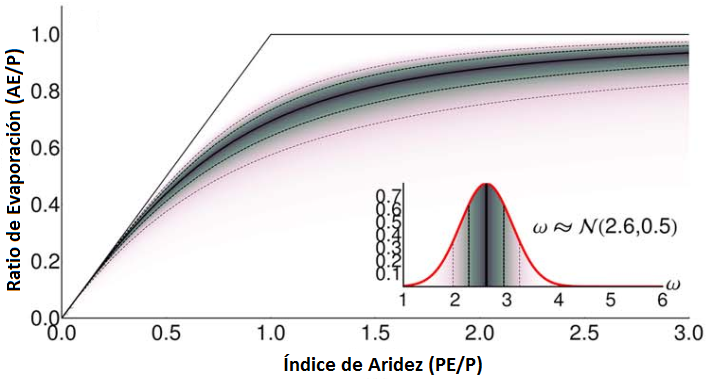
\includegraphics[scale=.75]{Images/Greve2015_prob_budyko.png}} \hfill
 \caption{a) Tradicional curva de Budyko (correspondiente a un $\omega = 2.6$ \citep{Fu1981,Zhang2004}, linea gris) ubicando por $\omega = 2.6 \pm 1$ (lineas delgadas). La distancia Euclidiana ($\delta$) entre las curvas es diferente para cada valor de $PE/P$. b) Enfoque probabilístico de la curva de Budyko para un $\omega$ siguiendo una distribución normal truncada. La mediana de la distribución es $\omega = 2.6$, que corresponde a la version tradicional (linea negra solida). Los cuantiles se muestran como sombra.}
 FUENTE: Modificado de \citet{Greve2015}.
 \label{fig:budyko02}
\end{figure}
